\hypertarget{theory}{%
\section{Theory}\label{theory}}

\hypertarget{bayesian-inference}{%
\subsection{Bayesian inference}\label{bayesian-inference}}

Bayesian inference approaches for modeling conformational ensembles
generally seek to model a \emph{posterior} distribution \(P(X|D)\) of
conformational states \(X\), given some experimental data \(D\).
According to Bayes' theorem, the posterior distribution is proportional
to a product of (1) a \emph{likelihood} function \(Q(D|X)\) of observing
the experimental data given a conformational state \(X\), and (2) a
\emph{prior} distribution \(P(X)\) representing any prior knowledge
about conformational states.

\[P(X|D) \propto Q(D|X) P(X)\]

Here, the prior \(P(X)\) comes from theoretical modeling, while the
likelihood \(Q(D|X)\) corresponds to experimental restraints, typically
in the form of some error model reflecting how well a given conformation
\(X\) agrees with experimental measurements. One can think of \(Q(D|X)\)
as a reweighting factor for the population of each state \(X\), and the
BICePs algorithm can be thought of as a way to reweight conformational
populations to agree with experimental knowledge.

In BICePs, the error model reflects both uncertainty in the experimental
measurements and heterogeneity in the conformational ensemble, (i.e. how
likely are the observables for conformation \(X\) to be away from the
ensemble-average measurement, either due to experimental noise or
conformational heterogeneity). These uncertainties are usually not known
\emph{a priori}, and must be treated as nuisance parameters \(\sigma\)
which can be modeled using some prior model \(P(\sigma)\):

\[P(X,\sigma | D) \propto Q(D|X,\sigma) P(X) P(\sigma)\]

Posterior sampling over \(X\) and \(\sigma\) using Markov Chain Monte
Carlo (MCMC) can then be used to determine the conformational
populations given the experimental restraints as
\(P(X|D) = \int P(X,\sigma | D) d\sigma\). Similarly, the posterior
distribution of the experimental uncertainty
\(P(\sigma | D) = \int P(X,\sigma | D) dX\) gives information about how
well the posterior conformational distribution agrees with the
experimental restraints.

\hypertarget{reference-potentials}{%
\subsection{Reference potentials}\label{reference-potentials}}

The correct implementation of reference potentials is an importance
advantage of the BICePs algorithm. The experimental data used to
construct the likelihood function comes from some set of
ensemble-averaged experimental observables
\(\mathbf{r} = (r_1, r_2, ..., r_N)\). Such observables are
low-dimensional projections of some high-dimensional state space \(X\),
and therefore these restraints in the space of observables need to be
treated as \emph{potentials of mean force}.\footnote{Olsson, S.;
  Frellsen, J.; Boomsma, W.; Mardia, K. V.; Hamelryck, T.
  \href{http://journals.plos.org/plosone/article?id=10.1371/journal.pone.0079439}{Inference
  of Structure Ensembles of Flexible Biomolecules from Sparse, Averaged
  Data.} PLoS One 2013, 8, e79439}\footnote{Olsson, S.; Boomsma, W.;
  Frellsen, J.; Bottaro, S.; Harder, T.; Ferkinghoff-Borg, J.;
  Hamelryck, T.
  \href{https://www.sciencedirect.com/science/article/pii/S1090780711003090?via\%3Dihub}{Generative
  Probabilistic Models Extend the Scope of Inferential Structure
  Determination.} J. Magn. Reson. 2011, 213, 182−186.}\footnote{Hamelryck,
  T.; Borg, M.; Paluszewski, M.; Paulsen, J.; Frellsen, J.; Andreetta,
  C.; Boomsma, W.; Bottaro, S.; Ferkinghoff-Borg, J.
  \href{http://journals.plos.org/plosone/article?id=10.1371/journal.pone.0013714}{Potentials
  of Mean Force for Protein Structure Prediction Vindicated, Formalized
  and Generalized.} PLoS One 2010, 5, e13714.}

\[P(X | D) \propto \bigg[ \frac{Q(\mathbf{r}(X)|D)}{Q_{\text{ref}}(\mathbf{r}(X))} \bigg] P(X)\]

The bracketed weighting function is now a ratio, with the numerator
\(Q(\mathbf{r}|D)\) being a likelihood function enforcing experimental
restraints in the space of observables, while the denominator
\(Q_{\text{ref}}(\mathbf{r})\) reflects some reference distribution for
possible values of the observables \(\mathbf{r}\) in the absence of any
experimental restraint information, such that
\(-\ln [Q(\mathbf{r}|D)/Q_{\text{ref}}(\mathbf{r})]\) is a potential of
mean force. Without reference potentials, a great deal of unnecessary
bias is introduced when many non-informative restraints are used.

As an example to illustrate the importance of reference potentials,
consider an experimental distance restraint applied to two residues of a
polypeptide chain (Figure 1). In the absence of any experimental
information, we assume a reference potential
\(Q_{\text{ref}}(\mathbf{r})\) corresponding to the end-to-end distance
of a random-coil polymer with a chain length equal to that of the
intervening residues. For residues near each other along the chain, a
short-distance restraint may have
\([Q(\mathbf{r}|D)/Q_{\text{ref}}(\mathbf{r})] \sim 1\), contributing
little or no information to refine the conformational ensemble. If the
residues are far apart along the chain, however, a short-distance
restraint can be highly informative, with
\([Q(\mathbf{r}|D)/Q_{\text{ref}}(\mathbf{r})]\) greatly rewarding small
distances where the reference potential \(Q_{\text{ref}}(\mathbf{r})\)
is small.

\begin{figure}
\centering
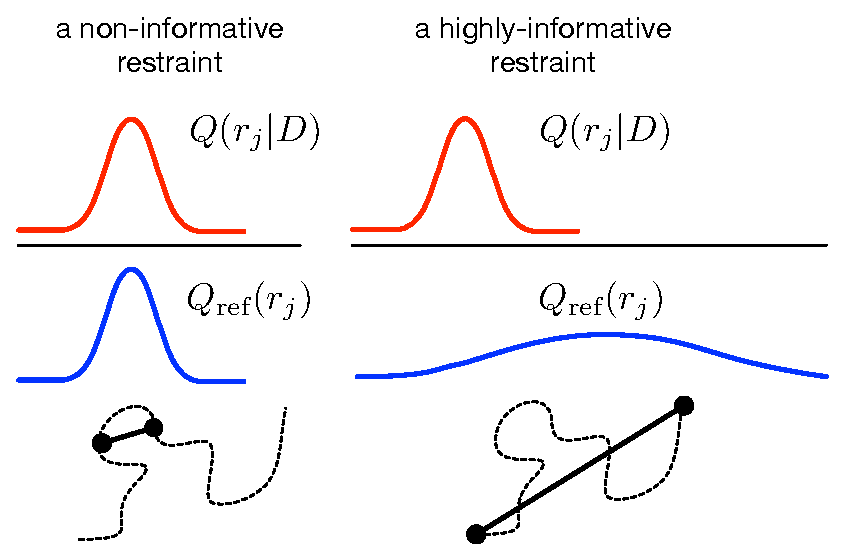
\includegraphics{figures/Figure1.pdf}
\caption{Figure 1.}
\end{figure}

\hypertarget{biceps-scores-for-quantitative-model-selection}{%
\subsection{BICePs scores for quantitative model
selection}\label{biceps-scores-for-quantitative-model-selection}}

Another key advantage of the BICePs algorithm is its the ability to use
the sampled posterior probability function to perform quantitative model
selection. This is done through a quantity we will call the *BICePs
score*.

Consider \(K\) different theoretical models \(P^{(k)}(X)\),
\(k=1,...,K\), that we may wish to use as our prior distribution.
Perhaps these models come from simulations using different potential
energy functions. Or perhaps we want to compare a model shaped only
experimental restraints, to a model using both simulation and
experimental information. Which model is more consistent with the
experimental data? To determine this, we compute the posterior
likelihood of the model, \(Z^{(k)}\), by integrating the \(k^{th}\)
posterior distribution across all conformations \(X\) and values of
\(\sigma\):

\[\begin{aligned}
Z^{(k)} = \int P^{(k)}(X,\sigma | D)  dX d\sigma  &=& \int P^{(k)}(X) Q(X) dX\\
 \text{total evidence for model } P^{(k)} && \text{overlap integral}
\end{aligned}\]

The quantity \(Z^{(k)}\) can be interpreted as the total evidence in
favor of a given model. Equivalently, we can think of this term as an
overlap integral between the prior \(P^{(k)}(X)\) and a likelihood
function
\(Q(X) = \int [Q(\mathbf{r}(X)|D,\sigma)/Q_{\text{ref}}(\mathbf{r}(X)) ] P(\sigma) d\sigma\).
The overlap integral quantifies how well the theoretical modeling agrees
with the experimental data (Figure 2); i.e. the value of \(Z^{(k)}\) is
maximal when \(P^{(k)}(X)\) most closely matches the likelihood
distribution \(Q(X)\) specified by the experimental restraints.

\begin{figure}
\centering
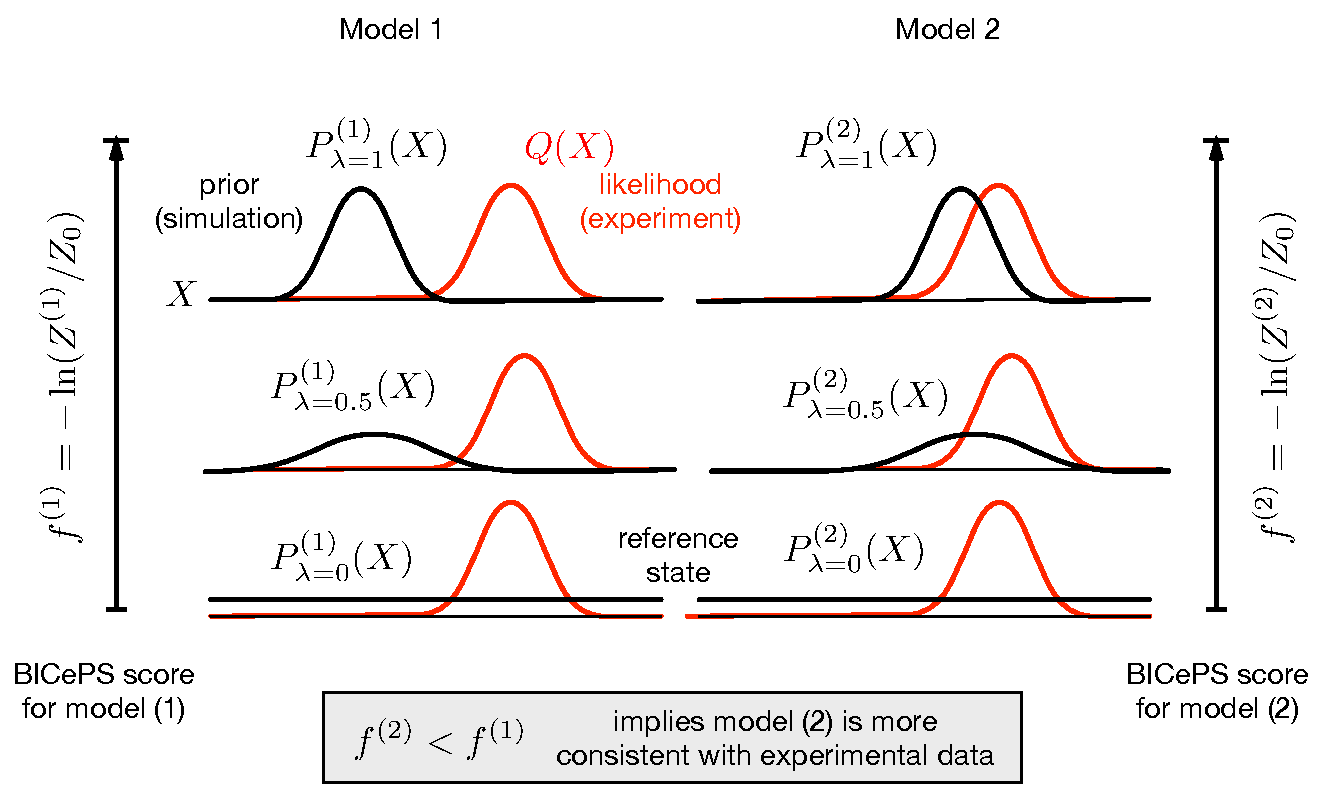
\includegraphics{figures/Figure2.pdf}
\caption{Figure 2.}
\end{figure}

In Bayesian statistics, the so-called Bayes factor, \(Z^{(1)}/Z^{(2)}\)
is a likelihood ratio that can be used to choose between competing
models (1) and (2), similar to a likelihood-ratio test in classical
statistics. In order to assign each model a unique score, we define a
free energy-like quantity,

\[f^{(k)} = -\ln \frac{Z^{(k)}}{Z_0}\]

to compare model \(P^{(k)}(X,\sigma|D)\) against some reference model
\(Z_0\). In practice, we choose the reference model to be the posterior
for a uniform prior \(P(X)\), i.e. no information from theoretical
modeling. We call \(f^{(k)}\) the BICePs score. The BICePs score
provides an unequivocal measure of model quality, to be used for
objective model selection. The lower the BICePs score, the better the
model (Figure 2). This useful property means that the BICePs score can
be used a metric for force field validation and parameterization. In
addition, the BICePs score has a useful physical interpretation: it
reflects the improvement (or disimprovement) of the posterior
distribution when going from a conformation ensemble shaped only
experimental constraints, to a new distribution additionally shaped by a
theoretical model.

\hypertarget{summary-of-the-key-advantages-of-biceps.}{%
\subsection{Summary of the key advantages of
BICePs.}\label{summary-of-the-key-advantages-of-biceps.}}

To put the BICePs algorithm in a larger context, we summarize the its
key advantages as follows:

\begin{itemize}
\tightlist
\item
  BICePs can be used with molecular dynamics (MD) or quantum mechanics
  (QM) methods. Conformational states can be individual conformations
  (like single-point QM minima) or collections of conformations (e.g.
  from clustering of trajectory data), as long as experimental
  observables can be attached to each conformational state.
\item
  BICePs performs reweighting of conformational states derived from
  modeling; it is currently a post-processing algorithm (MCMC) with no
  additional MD or QM required.
\item
  Bayesian inference offers a rigorous statistical framework for
  achieving the correct balance of theoretical modeling and experimental
  data.
\item
  BICePs correctly uses reference potentials, which is essential to
  proper weighing of experimental restraints
\item
  With proper reference potentials, BICePs scores can be used for
  unambiguous, objective model selection.
\end{itemize}

For more details about theory beneath BICePs, please check these
work.\footnote{Voelz, V. A.; Zhou, G.
  \href{https://onlinelibrary.wiley.com/doi/abs/10.1002/jcc.23738}{Bayesian
  Inference of Conformational State Populations from Computational
  Models and Sparse Exper- imental Observables.} J. Comput. Chem. 2014,
  35, 2215−2224.}\footnote{Yunhui Ge and Vincent A. Voelz,
  \href{https://pubs.acs.org/doi/10.1021/acs.jpcb.7b11871}{Model
  selection using BICePs: A Bayesian approach to force field validation
  and parameterization} Journal of Physical Chemistry B (2018) 122 (21):
  5610--5622}

\hypertarget{references}{%
\subsection{References}\label{references}}
